\section{Durchführung}
\label{sec:Durchführung}


\renewcommand{\labelenumi}{\alph{enumi})}
\begin{enumerate}
  \item Es soll die Zeitkonstante $\tau$ durch Beobachtung eines Auf- oder Entladevorgangs
  des Kondensators bestimmt werden. Die Schaltung wird gemäß Abb. 4 aufgebaut. Am Generator wird eine Rechteckspannung gewählt.
  Anschließend wird die Frequenz der Generatorspannung und des Oszilloskops auf einen
  geeigneten Bereich eingestellt, sodass der Graph eine fast vollständige Auf- oder Entladung darstellt. Zuletzt wird ein Bild des Graphen für die
  Auswertung gespeichert. Für diese werden dem Graphen einige Wertepaare entnommen und in einem
  halblogarithmischen Diagramm dargestellt. Zur Bestimmung von $\tau$ wird eine
  lineare Ausgleichsrechnung mit $\{(t, ln(U_C))\}$ durchgeführt, für dessen Steigung nach (4) gilt:
  \begin{equation}
  a = -\frac{1}{RC}
  \end{equation}
  \begin{figure}[H]
  	\centering
  	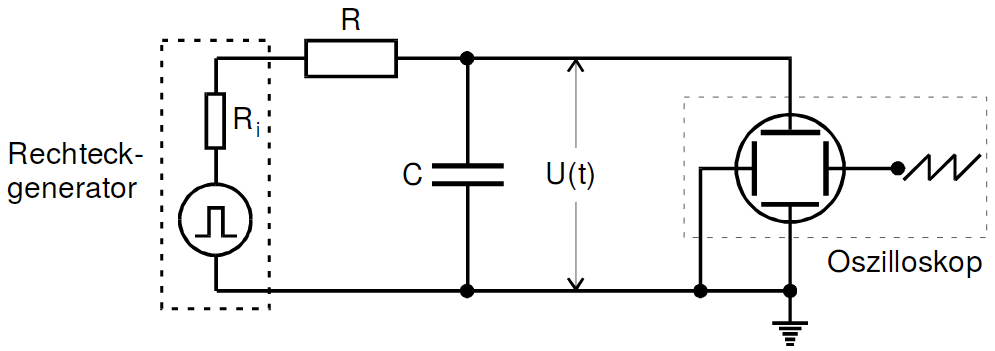
\includegraphics[width=\linewidth-200pt,height=\textheight-200pt,keepaspectratio]{content/Aufgabea.png}
  	\caption{Messchaltung zum Aufgabenteil a) \cite{V353}}
  	\label{fig:Aufbaua}
  \end{figure}

  \item Es wird die Amplitude A von $U_C$ an einem RC-Glied, welches an einem Sinusgenerator
   angeschlossen ist (Abb. 3), in Abhängigkeit von der Frequenz gemessen. Hierzu wird über
   3 Zehnerpotenzen hinweg variiert. Zur Auswertung wird $\{(f_{\text{Antrieb}}, A(f_{\text{Antrieb}}))\}$
   in einem halblogarithmischen Diagramm aufgetragen. Anschließend werden $\tau$ und $U_0$ mithilfe einer nichtlinearen
    Ausgleichsrechnung ermittelt. Mithilfe dieser wird die Theoriekurve nach (7) erstellt und
    ebenfalls eingetragen. Es soll diskutiert werden, ob eine systematische Abweichungen
    zwischen dem $\tau$ aus a) und dem aus b) existiert.
	\begin{figure}[H]
		\centering
		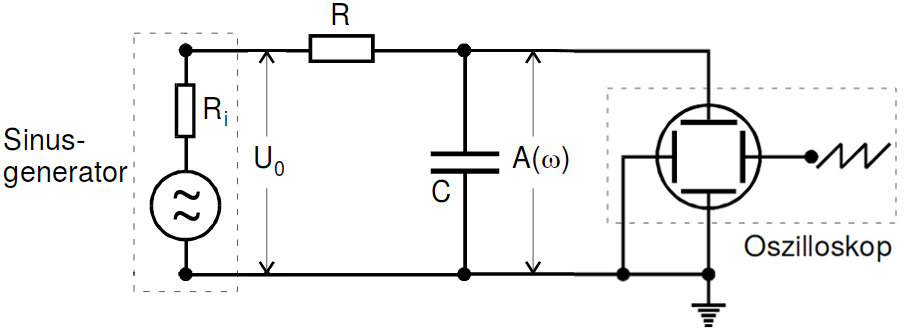
\includegraphics[width=\linewidth-200pt,height=\textheight-200pt,keepaspectratio]{content/Aufgabeb.png}
		\caption{Messchaltung zum Aufgabenteil b) \cite{V353}}
		\label{fig:Aufbaua}
	\end{figure}


    \item Es wird die Phasenverschiebung zwischen $U_{Antrieb}$ und $U_C$ an einem
    RC-Glied in Abhängigkeit von $f_{Antrieb}$ gemessen. Hierzu wird ein Zweikanaloszilloskop
    einmal über den Ausgang am Kondensator und einmal direkt an den Sinusgenerator angeschlossen (siehe Abb. 4)
     und so eingestellt, dass beide Graphen übereinander liegen. Es werden jeweils
      $\Delta t$ zwischen den Nullstellen und die zugehörige Frequenz notiert. Die jeweilige
       Phasendifferenz berechnet sich mit:
       \begin{equation}
         \varphi = 2 \pi \cdot \Delta t \cdot f_{Antrieb}
       \end{equation}
       Für die Auswertung wird mit der Menge der Messertpaare $\{(f_{Antrieb}, \varphi(f_{Antrieb}))\}$
       analog wie in Teil b) verfahren.
       \begin{figure}[H]
       	\centering
       	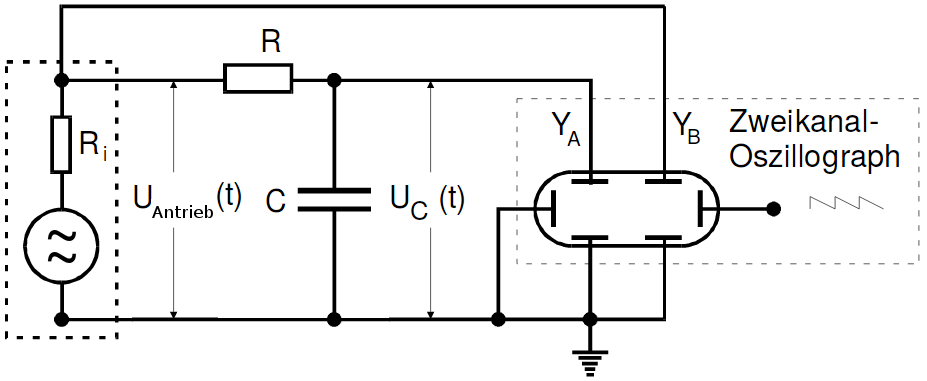
\includegraphics[width=\linewidth-200pt,height=\textheight-200pt,keepaspectratio]{content/Aufgabec.png}
       	\caption{Messchaltung zu den Aufgabenteile c) und d) \cite{V353}}
       	\label{fig:Aufbaua}
       \end{figure}

	\item Es wird die Relativamplitude $A(\omega) / U_0$ in Abhängigkeit von $\varphi$ in einem Polarkoordinatensystem dargestellt.
	Dies folgt aus Formel (7) und (8):
	\begin{equation}
	A(\varphi) = -U_0\cdot sin(\varphi)\sqrt{\frac{1}{sin^2(\varphi)}-1}\text{.}
	\end{equation}
	Zusätzlich werden auch einige Messwertpaare $(\varphi(\omega_i), A(\omega_i)/U_0)$ in das Diagramm
	eingetragen.

       \item Zuletzt soll gezeigt werden, dass der RC-Kreis nach den Voraussetzungen aus 2.4 als
       Integrator arbeiten kann. Die Schaltung bleibt dieselbe, wie bei Aufgabenteil c).
       Anschließend wird eine hochfrequente Spannung am Generator gewählt und das Oszilloskop so eingestellt, dass
       die zu integrierende und die integrierte Spannung dargestellt werden. Zum Vergleich werden
       Bilder der Graphen erstellt.



\end{enumerate}
